% --------------------------------------------------------------
% This is all preamble stuff that you don't have to worry about.
% Head down to where it says "Start here"
% --------------------------------------------------------------
 
\documentclass[12pt]{article}

\usepackage[margin=1in]{geometry} 
\usepackage{amsmath,amsthm,amssymb}
%\usepackage[spanish]{babel} %Castellanización
\usepackage[T1]{fontenc} %escribe lo del teclado
\usepackage[utf8]{inputenc} %Reconoce algunos símbolos
\usepackage{lmodern} %optimiza algunas fuentes
\usepackage{graphicx}
\graphicspath{ {images/} }
\usepackage{hyperref} % Uso de links
 \usepackage[most]{tcolorbox}
 \usepackage{lmodern}
\newcommand{\N}{\mathbb{N}}
\newcommand{\Z}{\mathbb{Z}}
 \usepackage{fancyhdr}
\usepackage{listings}
\usepackage{xcolor}
\usepackage{parskip} 
\usepackage{mathpazo} 

\definecolor{codegreen}{rgb}{0,0.6,0}
\definecolor{codegray}{rgb}{0.5,0.5,0.5}
\definecolor{codepurple}{rgb}{0.58,0,0.82}
\definecolor{backcolour}{rgb}{0.95,0.95,0.92}

\lstdefinestyle{mystyle}{
    backgroundcolor=\color{backcolour},   
    commentstyle=\color{codegreen},
    keywordstyle=\color{magenta},
    numberstyle=\tiny\color{codegray},
    stringstyle=\color{codepurple},
    basicstyle=\ttfamily\footnotesize,
    breakatwhitespace=false,         
    breaklines=true,                 
    captionpos=b,                    
    keepspaces=true,                 
    numbers=left,                    
    numbersep=5pt,                  
    showspaces=false,                
    showstringspaces=false,
    showtabs=false,                  
    tabsize=2
}

\lstset{style=mystyle}

 
\begin{document}
 
% --------------------------------------------------------------
%                         Start here
% --------------------------------------------------------------
 
\title{APS 105: Computer Fundamentals}
\date{}
\author{Tutorial \#5\\ 
Summer 2025}

\maketitle

\section*{Problem 1: Last String in String ( Winter 2022 Final Exam, Q10)}

Write a function called \texttt{lastStringInString}, the prototype of which is provided below, that returns the pointer to the last occurrence of the string \texttt{s1} in the string \texttt{s2}. If the string \texttt{s1} cannot be found in the string \texttt{s2}, the function returns \texttt{NULL}. For example, if we are looking for the string ``is'' as \texttt{s1} in the string ``This is a sample string'' as \texttt{s2}, the pointer to the second ``is'' in the string \texttt{s2} will be returned by the function. Another example, if we are looking for the string ``the'' as \texttt{s1} in the string \texttt{s2} ``The apple'', the function should return \texttt{NULL}. This is because `t' is lower case in ``the''.

Note: You can use any function from the library \texttt{string.h}, except for \texttt{strstr}() { you are not allowed to use it.
	
	
\textbf{Function Prototype:}
\begin{lstlisting}[language=C]
char *lastStringInString(char *s1, char *s2) 
\end{lstlisting}
	

\textbf{Example solution:}
\begin{lstlisting}[language=C]
char * lastStringInString ( char * s1 , char * s2) {
	char * p = s2;
	char * lastFound = NULL ;
	// Alternatively , we can write the while loop as:
	// while ( endOfString - p >= strlen (s2 ))
	// while ( strlen (p) - str (s1) >= 0)
	while (*p != '\0 ') {
		if ( strncmp (s1 , p, strlen (s1 )) == 0) {
		lastFound = p;
		}
		p++;
	}
	return lastFound ;
}
\end{lstlisting}

\section*{Problem 2:Declare and Initialize Struct (Winter 2024  Final Exam, Q2)}
Given the following defined data structure, write a single C statement terminated by one $;$, that declares a variable named $p1$ of the type of the following data structure. In the same statement, initialize the variable such that the value of $x$ is $1$,the value of  $y$ is $2$, and the value of $z$ is $3$.

\begin{lstlisting}[language=C]
typedef struct point {
	int z;
	int y;
	int x;
}
\end{lstlisting}

\textbf{Example solution:}
\begin{lstlisting}[language=C]
p1={3, 2, 1}
\end{lstlisting}

\section*{Problem 3: Fixing Memory Issues (Winter 2024 Final Exam, Q5)}
The C program given below does not produce the expected output. You will be asked to fix the code in two specific parts, (a) and (b), as described below. The expected output is:

\begin{tcolorbox}[colback=gray!10, boxrule=0pt, sharp corners, enhanced jigsaw, left=3mm, right=3mm, top=1mm, bottom=1mm]
Enter last name: Patel\\
Enter last name: Wang\\
Patel\\
Wang\\
\end{tcolorbox}

The program takes in two names from the user and saves them in the \texttt{lastName} member in the array of data structures students. However, the program does not produce the expected output. In the code below:
\begin{enumerate}
	\item In (a) replace the line \texttt{students[i].lastName = str;} with code that results in the expected output. You may assume the maximum string size is $20$ and the \texttt{stdlib.h} is included.
	\item In (b) dynamically deallocate using free function any dynamically allocated data in the code. 
\end{enumerate}

The C program is:
\begin{lstlisting}[language=C]
typedef struct student {
	char* lastName; 
} Student;

void getNames(Student students[]) { 
	char str [20];
	for (int i = 0; i < 2; i++) {
		printf("Enter last name: "); 
		scanf("%s", str);
		// TO BE COMPLETED
		// (a): Correct the following line 
	students[i].lastName = str;
	}
}

int main(void) {
	Student* students = (Student*)malloc(2 * sizeof(Student));
	getNames(students);
	for (int i = 0; i < 2; i++) {
		printf("%s\n", students[i].lastName);
	}
	// TO BE COMPLETED
	// (b): Deallocate dynamically allocated memory
}
\end{lstlisting}

\textbf{Example solution:}
\begin{lstlisting}[language=C]
// a
students[i].lastName = (char*) malloc(sizeof(char) * 20); 
strcpy(students[i].lastName , str);

// b
for(int i = 0; i < 2; i++){ 
	free(students[i].lastName);
} 
free(students);
\end{lstlisting}

\section*{Problem 4: Reomve the Tail Node (Winter 2024 Final, Q7)}

The following code intends to remove the tail node in a linked list. Complete the removeTail function such that the last node is removed, properly freed and no segmentation fault is caused. The data structure definition of LinkedList and Node are shown below.


\begin{lstlisting}[language=C]
typedef struct node { 
	int data;
	struct node* next;
} Node;

typedef struct linkedList { 
	Node* head;
} LinkedList;

void removeTail(LinkedList* list) { 
	Node* current = list ->head;
	Node* prev = NULL;
	if (list ->head == NULL) {
		return; 
	}
	while (current ->next != NULL) { 
		prev = current;
		current = current ->next;
	} 
}
\end{lstlisting}

\textbf{Example solution:}
\begin{lstlisting}[language=C]
void removeTail(LinkedList* list) { 
	Node* current = list ->head;
	Node* prev = NULL;
	if (list ->head == NULL) {
		return; 
	}
	while (current ->next != NULL) { 
		prev = current;
		current = current ->next;
	} 
	
	// Solution:
	if (list ->head ->next !=NULL){
		free(current);
		prev ->next = NULL;
	} else { 
		free(current);
		list ->head = NULL;
	}
}
\end{lstlisting}

\section*{Problem 5:  Linkedlists Iscycle ( Winter 2024 Final, Q11)}

The Node structure in a linked list has been defined as follows:
\begin{lstlisting}[language=C]
typedef struct node { 
	int data;
	struct node *next;
} Node;
\end{lstlisting}
The LinkedList structure has also been defined to contain the head of a linked list:
\begin{lstlisting}[language=C]
typedef struct linkedList { 
	 Node *head;
} LinkedList;
\end{lstlisting}
We have learned in class that the tail node in the linked list has its next pointer point to \texttt{NULL}. In a linked list with a cycle, the tail node next points to the head node in the linked list. Write a C function named \texttt{isCycle}, the prototype of which is given below, that takes \texttt{LinkedList*} list as an argument and returns true if there exists a cycle, otherwise, it returns false.

\textbf{Example solution:}
\begin{lstlisting}[language=C]
bool isCycle(LinkedList* list) { 
	Node* current = list ->head;
	if (current != NULL) { // if there is a next node, look at it 
		current = current ->next;
}
	while (current != NULL && current != list->head) {
		current = current ->next; 
	}
	return (current == list->head); 
}
\end{lstlisting}



\section*{Problem 6: Doubly Linked Lists (Winter 2025 Final Exam, Q32)}
Another category of linked lists called \textbf{doubly linked lists} has each node store \texttt{data}, which is an integer value, \texttt{prev}, which is a pointer to the previous node and \texttt{next}, which is a pointer to the next node. This makes it easier to traverse the list in both directions.

The definition of a node in a doubly linked list is provided below:

\textbf{Function Prototype:}
\begin{lstlisting}[language=C]
// Struct for a node in the doubly linked list
typedef struct node{
	int data;
	struct node* prev;
	struct node* next;
} Node;

// Struct for the linked list
typedef struct{
	Node* head;
	Node* tail;
} DoublyLinkedList;
\end{lstlisting}

You are required to implement the function \texttt{insertAfterNode}, the prototype of which is shown below, that inserts a new node \textbf{after} a given node in a doubly linked list as shown in the figure below. \texttt{list} is a pointer to the doubly linked list, \texttt{prevNode} is a pointer to node after which you'd need to add a new node, and \texttt{val} is the value of the data member of the new node that you're required to dynamically allocate and insert in the list. You can assume \texttt{prevNode} will be pointing to a valid node.

\begin{figure}[h]
	\centering
	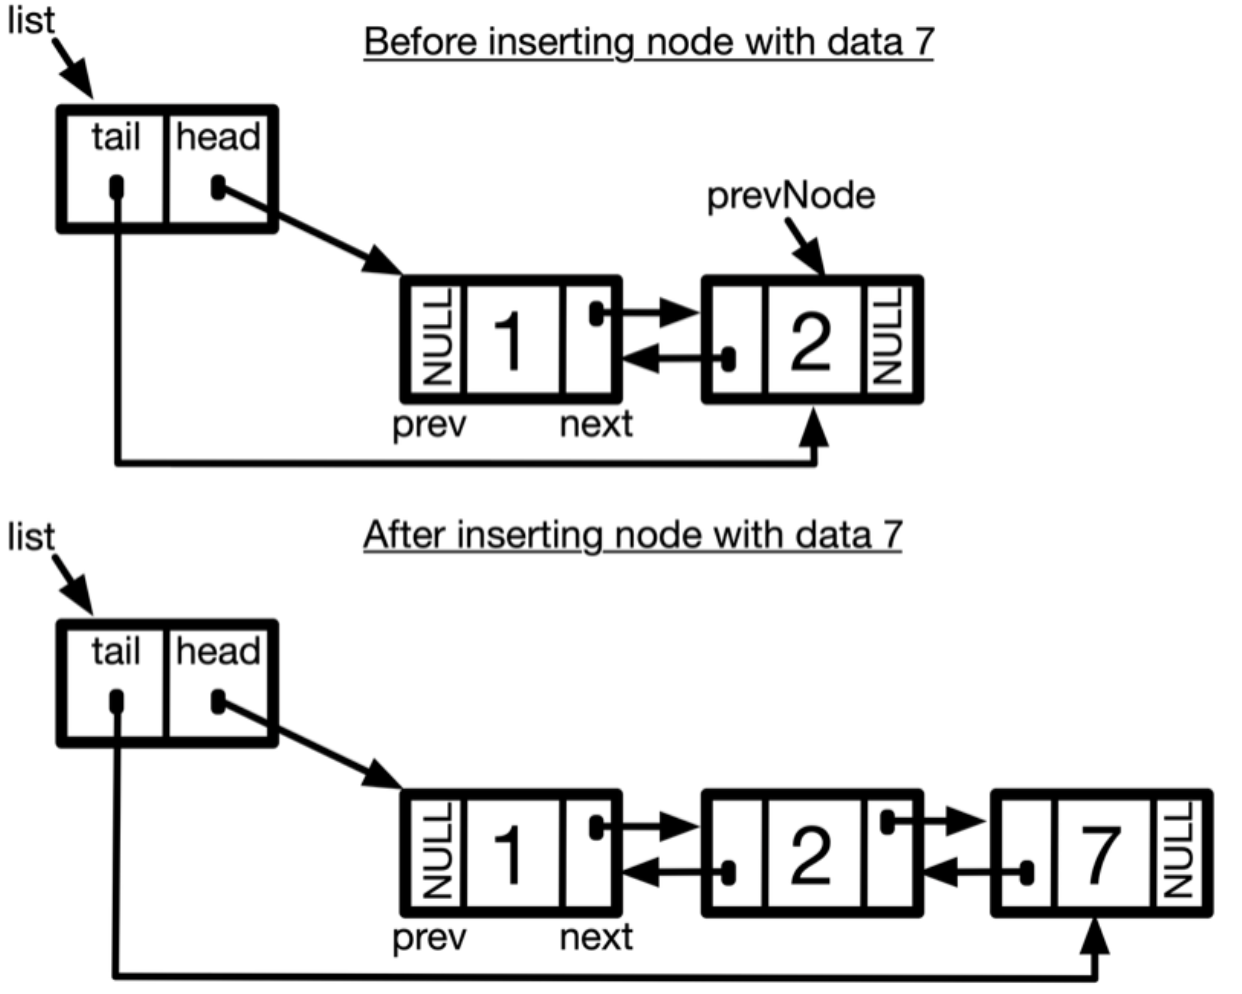
\includegraphics[width=0.5\textwidth]{./doubly.png}  % Replace with your image file name
	\caption{Examples of the doubly linked lists.}
\end{figure}
Note that in a doubly linked list, we are required to also keep track of the last node in the list, also known as the tail.
\begin{lstlisting}[language=C]
	void insertAfterNode{DoublyLinkedList* list, Node* prevNode, int val};
\end{lstlisting}

\textbf{Example solution:}
\begin{lstlisting}[language=C]
void insertAfterNode(DoublyLinkedList *list, Node *prevNode, int val)
{
    // Create the new node
    Node *newNode = (Node *)malloc(sizeof(Node));
    newNode->data = val;
    newNode->prev = prevNode;

    // If newNode is not the last node, update the prev of the next node
    if (prevNode->next != NULL)
    {
        newNode->next = prevNode->next;
        prevNode->next = newNode;
        newNode->next->prev = newNode;
    }
    else
    {
        prevNode->next = newNode;
        newNode->next = NULL;
        // If newNode is the last node, update the tail pointer
        list->tail = newNode;
    }
}
\end{lstlisting}

\end{document}